\documentclass[conference]{IEEEtran}
\IEEEoverridecommandlockouts
% The preceding line is only needed to identify funding in the first footnote. If that is unneeded, please comment it out.
\usepackage{cite}
\usepackage{amsmath,amssymb,amsfonts}
\usepackage{algorithmic}
\usepackage{graphicx}
\usepackage{textcomp}
\usepackage{xcolor}
\usepackage{array}
\def\BibTeX{{\rm B\kern-.05em{\sc i\kern-.025em b}\kern-.08em
    T\kern-.1667em\lower.7ex\hbox{E}\kern-.125emX}}
\usepackage[caption=false,font=footnotesize]{subfig}

\begin{document}
\graphicspath{{images/}}
% and their extensions so you won't have to specify these with
% every instance of \includegraphics
% \DeclareGraphicsExtensions{.pdf,.jpeg,.png}

\title{Oil Well Monitoring and Production Forecast with Artificial Intelligence using System Identification techniques}

\author{\IEEEauthorblockN{Anonymous Authors}}

\maketitle

\begin{abstract}
In the oil and gas industry, long-term development strategies as well as short-term operational decisions rely on well monitoring data. In recent years, this industry has benefited from machine learning techniques as the availability and quality of oil field data, allowing the application of data-driven models to fit and predict field behaviour and provide better business decisions. Among the variables of interest, the production rates are worth studying due to its connection to the revenue and uncertainties associated to its determination.

This study provides a system identification approach to create black-box estimators to predict production rates in oil wells by using control settings and sensor data from the well. One well from the Volve dataset was chosen as the benchmark and a python-implemented class was deployed in order to use sklearn-compatible regressor to perform the adjust. A comparison of a neural network with more classical estimators fore system identification is performed for single input and multiple input cases with the best lag order selection and hyperparameter randomized search being performed for each case.

The final models showed interesting results when compared to the real data, with the MLP outperforming the more classical models and the multiple input cases outperforming the single input cases. single input MLP was also noted as an alternative to reduce the dependency of well sensors and the multiple input NARX-equivalent method was noted as an alternative for cases where computational resources might be an issue.

%This study provides a black box system identification approach to overcome these limitations and address the well monitoring challenges, being an alternative to conventional well flow rates estimation and pressure-temperature gauges unavailability. We focused in well flow rates estimation based on operational available input data and aiming missing production history, reservoir management and production forecast applications: a digital twin for an oil well.

%A python implemented class was deployed in order to allow the use of any standard regressor to predict time series values, once a set of input/output lags is selected. This flexibility improves the implementation of those models and makes the comparison between model types more feasible. The MLP regressor, as well as other types of regressors showed a good accuracy in predicting rates for a real field well application, where the dynamics are difficult to predict due to the wide range of operational conditions.
\end{abstract}

\begin{IEEEkeywords}
system identification, scikit-learn, neural network, oil and gas, production forecast, digital twin.
\end{IEEEkeywords}

\section{Introduction}\label{section_introduction}
% no \IEEEPARstart

% INTRODUCAO
%\color{black}
Well monitoring and production rates estimations compose the reservoir management activity 
and have a major role in the oil and gas industry. Being able to accurately forecast the 
production of a well or an oilfield is a constant need on the oil and gas industry in order 
to assess the economic value of its assets, calculate royalties to be paid and perform an 
effective reservoir management strategy that will increase the value extracted from the oil 
field \cite{alakeely2022simulating}.

In most offshore production facilities, the separation of the three phases (oil, gas and water)
of the wells is performed only for the total production of the unit, as the space available 
for the separation vessels is limited. A second separation system is usually available to 
separate fluids of a single well in order to have an accurate measurement of its three phases 
flow rates. This vessel is called test separator and this operation of measuring flow rates is 
known as well test. As the separator test measures are obtained for a single well at a time, 
most part of the time the well flow rates are not being continuously acquired. The full 
historic production flow rates for each of the connected wells, is then, uncertain as it 
is usualy reported as an apportionment of the total production. An alternative to the 
traditional well test based apportionment is the use of multi phase flow meters, however, 
since multi phase flow is complex, turbulent, and chaotic, the acquisition of accurate, 
reliable, and repeatable rate measurements can be a challenge \cite{Okotie2016}.

Due to the challenges associated to the determination and forecasting of production rates per 
well, production predictions are normally performed by using simulation models based on first 
principles. These models are built and maintained by qualified engineers by using pressure and 
temperature data taken from sensors positioned in key points of the well, some of which are 
displayed schematically in figure \ref{fig:pressureSensors}. Adjusting the reservoir model in 
order to correctly match the actual dynamic historic behaviour is the process known as history 
match \cite{alakeely2022simulating}. Li et al. \cite{Li2019} comment that this approach, due 
to some simplified assumptions, may generate uncertain models and also cites the pressure 
dependency of the flow rate as input, an already uncertain variable, as a major limitation. 
Cao et al. \cite{CaoQ2016} also comments that, specially for unconventional resources, a 
conventional characterization of the field may not be feasible thanks to ultra-tight shale 
formations for some unconventional fields, uncertainties in the geological properties and 
heterogeneous rock formations, being the last two challenges commonly found even in more 
conventional assets. The dependency of well sensors for the history match can also be a 
challenge, since there is always a risk of losing some measurements. As an example, the 
donwhole pressure is one of the most important variable to provide useful information for 
management and oil recovery of the oil field \cite{camponogara2010automation} but the PDG 
sensor responsible for its measurement has a high failure rate. Those systems for measuring 
pressure and temperature historically exhibited a low reliability \cite{Gisbergen2001} and, 
in offshore wells, the replacement of such equipment once it's damaged is not a common 
operation due to the high costs associated with the workover operation and high environmental 
risks \cite{Freitas2021}. In that case, reservoir management becomes more challenging and lack 
of information may hinder decisions that depend on long-term predictions. 

\begin{figure}[htbp]
\centerline{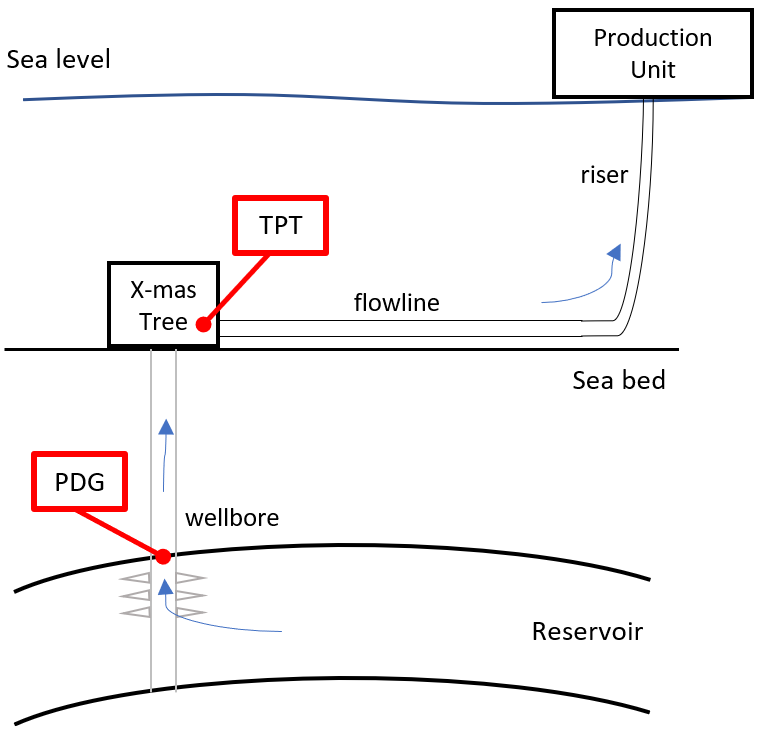
\includegraphics[width=3.0in]{wellScheme.png}}
\caption{Typical offshore well and its pressure-temperature sensors: PDG (located downhole) and TPT (located in the X-mas tree, the sea bed equipment which connects the well with the flowline).}
\label{fig:pressureSensors}
\end{figure}

% LITERATURE REVIEW
Reservoir management area has recently benefited from machine learning methods that emerged as 
powerful tools to address these key challenges \cite{alakeely2022simulating}, posing as an 
alternative to the conventional first principles approach. Many studies have addressed the 
problem of predicting well rates and reservoir monitoring by the use of artificial intelligence 
techniques such as machine learning methods. According to Alakeely et al. \cite{AlakeelyGA2022}, these models are powerful tools for tasks where the actual model between the input and output variables is not well defined or does not exist, and where forward modeling is well defined, but the inverse model is challenging. The difficulty in modeling the dynamic behaviour of those systems is that they present a wide range of operating conditions what makes the prediction task a challenging one \cite{Freitas2021} \cite{Apio2019}. This happens because the physical phenomena that happen in a certain time window on a well production history are not expected to be repeated over time as the water and gas fractions tend to rise and the pressure levels tend to monotonically decrease. These variables are responsible for changing the well behavior in several parameters, like productivity index, phase viscosities and densities. 

Alakeely and Horne \cite{Alakeely2021} proposed a Deep Learning method using surface measurements 
to predict well flow rates. Also in \cite{Alakeely2021}, autoencoders were used to generate 
additional inputs and the results were compared to classic Gilbert correlation methods. 
Cao et al. \cite{CaoQ2016} used a single-layer fully-connected neural network to predict the 
production rates of existing wells, but also tried o add information from the geologic contex 
in order to predict new wells.

As already mentioned, well pressure and temperature sensors, in case of fail, are unlikely to 
be replaced in a short period thanks to economical and environmental reasons. In that sense, 
soft sensors models emerge as an alternative to replace a sensors such as the PDG 
\cite{Aguirre2017}. A study on PDG soft sensors is provided by Aguirre et al. in 
\cite{Aguirre2017} using NARMAX, neural networks, committee machines, unscented Kalman filters 
and filter banks models. Aguirre et al. \cite{Aguirre2017} also show the key-problems in 
developing soft-sensors and reveal the strengths and weaknesses of each alternative, based on 
diverse oil wells considered. An application of Echo State Network to model well downhole and 
riser inlet pressure by using surface and subsea valves position as input variables is 
provided by Jourdanou et al. \cite{JORDANOU2019} where the data is generated by a flow 
simulator and the framework is then used for nonlinear model predictive control (NMPC) 
purposes. Li et al. \cite{Li2019} also modeled the downhole pressure with deep learning 
models, searching for the best architecture to represent short-term transients and long-term 
variations. %, but also using the rates as inputs.

A black-box identification procedure consists of using only data set available input and output 
information. Freitas et al. \cite{Freitas2021} propose the use of steady-state response as an 
additional information to improve the quality of the model predictions, creating gray-box 
models that outperformed the black-box ones in the cases studied by adding more physical 
information of the first principles. Similarly, Apio et al. \cite{Apio2019} propose the use of 
Kalman filters as gray-box models to expand the range of process operating conditions as MLP 
have poor results outside the train time window \cite{Apio2019}. In \cite{Liu2022} Liu et al. 
showed that Genetic Algorithms parameterized Echo State Networks were predictive in short term 
forecasts of three field cases. These auto-regressive models outperformed other machine learning 
model classes and proved to be efficient for missing flow history or short-term well performance 
forecast applications.

% Critial analysis, paper goals, and original contributions
The main goal of this work is to build a neural network based black-box model to predict well 
flow rates using available field measures like pressure gauges, surface valves positions and 
historical production data. Thereby, the data-driven methodology is intended to be the basis 
of a Digital Twin for an oil well as an alternative to production tests, first principles 
simulations or multiphase flowmeters, providing a useful tool to recover missing historical 
field data or optimize and forecast field production. Although this paper focuses on rate 
estimation, the techniques and framework proposed in this paper could be applicable to any 
desired variable.

This paper's objective is to some extent shared with the works of Alakeely and Horne 
\cite{Alakeely2021}, Liu et al. \cite{Liu2022} and Cao et al. \cite{CaoQ2016}, with the main 
contributions of adding a system identification approach to the problem with the selection of 
the best model order (lag), best input space and comparison with more classical system 
identification methods through the implementation of a Python-implemented class that easily 
performs time series regression by using any scikit-learn regressors. The application of 
randomized hyperparameter search and cross-validation to the models in order to perform 
hyperparameter tuning and evaluate computational performance and train set sensitivity is 
also part of the main contributions of this paper.

%The main contribution of this paper is the application in a real field well case with challenging dynamics to be identified and the methods capability to be easily generalized to any standard scikit learning regressor class.

% paper organization
This paper is organized as follows: in section \ref{section_case_study} we describe the case 
study, the dataset characteristics and the variables used. Also in section 
\ref{section_case_study}, a brief formulation of well rates estimates as a system 
identification problem is presented. In section \ref{section_method}, the methodology is 
detailed and in \ref{section_results} a discussion is conducted regarding the most important 
results achieved. Finally, a conclusion is made in section \ref{section_conclusion} as well as 
future works and analysis recommendation.


\section{Case study}\label{section_case_study}

The Volve field is an oilfield on the North Sea discovered in 1993. The field was operated by 
Equinor who started production in 2008 from a Middle Jurassic age sandstone reservoir 
\cite{volve_info}. The field was shut down on 2016, with its production facilities being 
removed in 2018.

An open-source dataset containing exploration and production data from this field, the Volve 
dataset, was then disclosed by operator Equinor, in 2018. The dataset contains geological, 
geophysical, seismic and logging data, reservoir models and reports from the Volve field 
\cite{volve_data}. The dataset also includes production data from the reservoir, 6 production 
wells and 1 injection well, which includes dynamic data of pressure and temperature sensors, 
choke sizes and production flow rates. Some of the variables available on the dataset for each 
production well and its definitions are listed on the table \ref{volve_variables}.

\begin{table}[htbp]
\caption{Volve Dataset variables and definitions used on this case}
\begin{center}
\centering
\begin{tabular}{|c|c|}
\hline
\textbf{Variable}&{\textbf{Definition}} \\
\hline
BORE\_OIL\_VOL             & Average oil flow rate on \\
                           &  one day of production\\
\hline
BORE\_WAT\_VOL             & Average water flow rate on \\
                           & one day of production\\
\hline
BORE\_GAS\_VOL             & Average gas flow rate on \\
                           & one day of production\\
\hline
BORE\_LIQ\_VOL            & Average liquid flow rate on \\
                           & one day of production\\
\hline
AVG\_DOWNHOLE               &  Daily average of the downhole\\             
\_PRESSURE                  &  pressure measured by the permanent\\
                            &  downhole gauge (PDG)\\
\hline
AVG\_DOWNHOLE               &   Daily average of the downhole\\
\_TEMPERATURE               &  temperature measured by the \\
                            &  permanent downhole gauge (PDG)\\
\hline
AVG\_WHP\_P                &   Daily average of the wellhead\\
                           &  pressure measured at the christmas\\
                           &  tree valve\\
\hline
AVG\_WHP\_T                &   Daily average of the wellhead\\
                           &  temperature measured at the \\
                           &  christmas tree valve\\
\hline
AVG\_CHOKE\_SIZE\_P        &   Daily average of the choke   \\
                           &   valve opening position (full \\
                           &   opening percentage)          \\
\hline
DP\_CHOKE\_SIZE            &   Daily average of the pressure \\
                           &   drop caused by the choke \\
\hline
AVG\_DP\_TUBING            &   Pressure difference between the\\
                           &   average downhole pressure and the \\
                           &   average wellhead pressure \\
\hline
\end{tabular}
\label{volve_variables}
\end{center}
\end{table}

As already established in section \ref{section_introduction}, flowrates are important variables 
to be estimated and predicted on a multiphase system, but also are difficult to be obtained 
directly. The standard approach regarding the prediction of these variables consists on 
creating, adjusting and maintaining simulation models based on first principles and using them 
to predict a well or an oilfield production throughout its life. As a general rule, at least 
two models, one that simulates the multiphase flow in the porous media and one that simulates 
it in wells and pipelines, are needed in order to predict the production rates. The main 
disadvantage of this approach is its great dependency of the interpretation of very uncertain 
data (such as geological data) and also great dependency of expert knowledge to decide which 
variables should be used in order to adjust the models.

Another valid approach to create a model for an oil field or an oil well is to understand that 
both these entities can be seen as dynamic systems, where it is known that the history of its 
controls (ex.: well chokes) and some state variables (ex.: pressure and temperature measurements) 
can be used to predict an output variable such as its liquid rate. As mentioned by Li et at. 
\cite{Li2019}, experience shows that the measured pressure and temperature variables in a well 
are related to its controls and flow rates. This black-box model can be achieved by applying a 
system identification approach for this problem assuming a discrete-time systems. This method 
has the disadvantages of needing some production history in order to create the model and also 
being very dependent of how dynamically rich this data is, but also has the great advantage of 
having a purely data-driven model that is less dependent of geological interpretations.

For this work, it was not selected as a case study the whole reservoir, hence only one well 
will be used. The well selected was the well 15/9-F-1 C from the Volve field and its main 
variables available on can be seen in figure \ref{example_well}. This well was selected 
because it has a rich dynamic behaviour, with multiples shut-ins throughout its life, making 
it an interesting case for creating a black-box model. It is worth mentioning that this well 
was also used by Li et al. \cite{Li2019} in his work about the application of Deep Learning 
for well history analysis, but his work was focused on predict the downhole pressure.

\begin{figure}[htbp]
\centerline{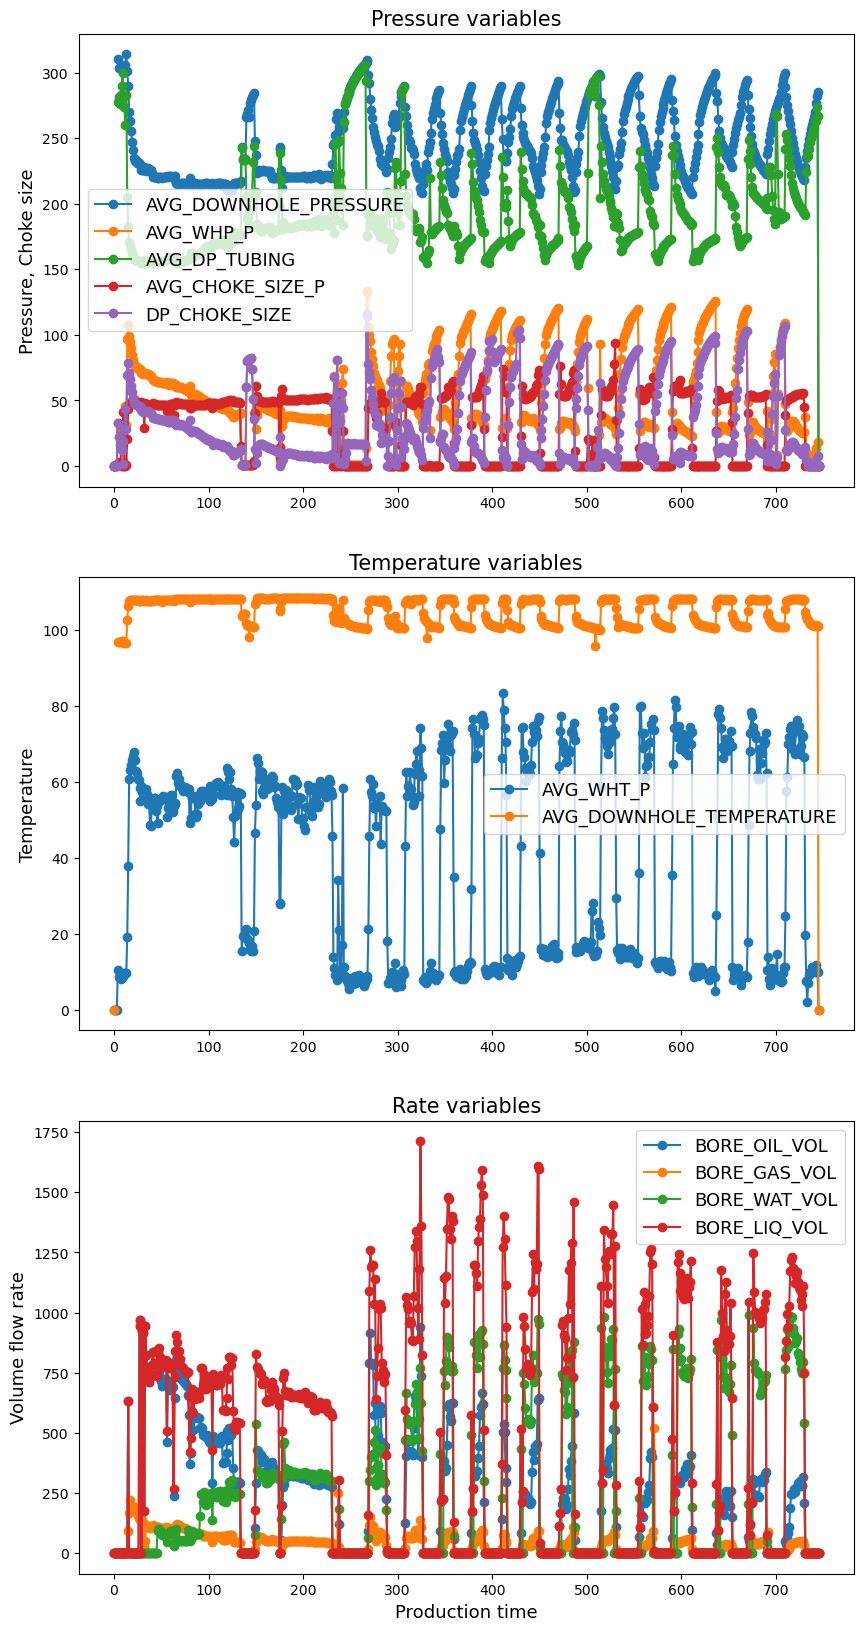
\includegraphics[width=3.5in]{data_example_2.png}}
\caption{Example of well production data available on Volve dataset}
\label{example_well}
\end{figure}

It is also interesting to notice that, since the variables are all daily averages, the 
discrete-time approach is valid and the time series has a constant time step of one day.

\section{Compared Methodology}\label{section_method}

In this section, the methodologies applied in this work in order to generate the results 
will be briefly described.

\subsection{System identification approach}

System identification consists on proposing a model (either black box or gray box) that is able
to correctly predict the behaviour of a dynamic system and perform forecasts. The approach tries 
to propose a regression model that can estimate the value of the output variable $y$ in the 
time instant $k$, as shown in equation \ref{eq:sysid_generic}

\begin{equation}\label{eq:sysid_generic}
    y_k = f(\mathbf{X}_{k-1})\,.
\end{equation}

Inspired by the control theory and discrete-time transfer functions, the input vector $\mathbf{X}$
is created by concatenating previous values of the input variable $u$ and the output variable $y$,
as illustrated in equation \ref{eq:sysid_generic}

\begin{equation}\label{eq:sysid_lags}
    \mathbf{X}_k = \
    \begin{bmatrix}
        u_{k} \\ u_{k-1} \\ ... \\ u_{k-n_u} \\ -y_{k} \\ -y_{k-1} \\ ... \\ -y_{k-n_y}
    \end{bmatrix}^T\,.
\end{equation}

When the regression function $f$ is linear, the method is called ARX (\textbf{A}uto\textbf{R}egressive
with E\textbf{X}ogenous variables). When the function is non-linear (usually a polynomial is used)
the method is called NARX (\textbf{N}on-linear ARX). Due to the generic nature of the function $f$,
any regressor (including fully-connected neural networks) can be used to create the model.

Among the advantages of the system identification approach it can be found the simplicity of the model,
its flexibility to different regressors. It is also important to comment that, even thoug equation \ref{eq:sysid_lags}
exemplifies the system identification approach with only a single input and a single output, multiple values of input and
output are also possible by adding more data to the
Some disadvantages of the approach include the need of data
with constant timestepping and, depending on the number of inputs, outputs and lag sizes, the amount of
memory spent in matrix $\mathbf{X}$ in order to store repeated data.

\subsection{Transformer architecture}

The method proposed in this study consists on applying a system identification approach to create a black-box model capable of simulate the dynamic behaviour of a production well. Since the time series has a constant timestep, this approach consists on finding a regressor capable of estimating the output variable by using a number of delayed values of the input and output variables, with the this number for each variable, in our case, being equal to a maximum lag provided as an input. After the creation of the regression vectors for each output value, any regression method can be used in order to create a model, with the more classical ones being a linear regressor (ARX model) and a polynomial regressor (Polynomial NARX model).

The basic pipeline performed on this work is shown in figure \ref{graphical_abstract}. In order to build the regression matrices using the defined lags, fit and predict using the fitted model, a Python class was implemented that allowed the use of any regressor from the scikit-learn (sklearn) \cite{scikit-learn} package to perform the regression of the model. The class also gives support for free-run simulations (where simulated outputs are used as input for the prediction of the next step) and one-step ahead simulations (where each predicted step uses real lagged outputs on this prediction). 

The production history from the selected well (15/9-F-1 C) was split into a train set composed of the first 70\% of the production history and a test set composed of the remaining 30\%. It was then normalized by ensuring that all the values on the train data would be contained on a [0, 1] interval. In order to evaluate the importance of using multiple sensors to fit the model, the train data was fed to the pipeline on a single input single output (SISO) schema, where only the choke size was used as an input variable, and on a multiple input single output (MISO) schema, where choke size and pressure and temperature data on the wellhead and bottom-hole were used as inputs.

\begin{figure*}[htbp]
\centerline{
\includegraphics[width=6.0in]{images/graphical_abstract.png}}
\caption{Graphical Abstract and Optimal model selection procedure}
\label{graphical_abstract}
\end{figure*}

As a mean to compare different regressors, three were selected and built using the sklearn available objects. These regressors are summarized in table \ref{regressors}. The  first two, LinReg and PolyReg, are equivalent to the classical ARX ans Polynomial NARX methods used in system identification. For the PolyReg model, it was assumed a polynomial degree of two for this study.

\begin{table}[htbp]
\caption{Scikit-learn regressors used for the system identification}
\begin{center}
\begin{tabular}{|c|c|}
\hline
\textbf{Method}&{\textbf{sklearn regressor}} \\
\hline
LinReg & LinearRegression  \\
\hline
PolyReg & PolynomialFeatures + LinearRegression   \\
\hline
MLP & MLPRegressor  \\
\hline
\end{tabular}
\label{regressors}
\end{center}
\end{table}

The third regressor used was a Neural Network built using the sklearn multi-layer perceptron (MLP) regressor and was chosen in order to compare the performance of a neural network with more classical approaches. Since the considered regressors all have hyperparameters that have to be chosen, a randomized search approach with cross-validation was adopted. This approach is also very useful because the cross-validation allows for the extraction of some statistical data regarding the impact of the train data on the model. For this work, a cross-validation with 5 folds and 10 iterations was used on the randomized search, that performed 100 iterations. 

In order to select the best lag orders, the randomized search was performed on different input matrices, built with different lag configurations. Accounting that free-run simulation is generally more useful for long term predictions, the best model selection was made based on the best R$^2$ score for the train data using the free-run simulation results. This metric is defined on equation \ref{r2_eq}, where $\mathbf{\hat{y}}$ represents a prediction vector and $\bar{y}$ represents the average value of the real output vector $\mathbf{y}$.

% \begin{figure}[htbp]
% \centerline{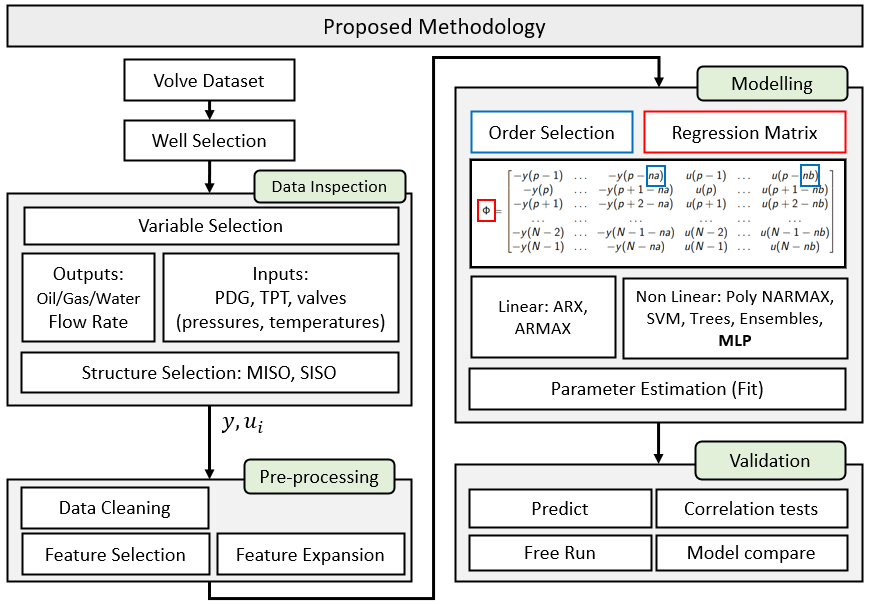
\includegraphics[width=3.5in]{graphical_abstract_2.png}}
% \caption{Main steps of the workflow}
% \label{graphical_abstract_2}
% \end{figure}


\begin{equation}\label{r2_eq}
    R^2 = 1 - \frac{\sum_{i=1}^N{(y_i - \hat{y}_i})^2}{\sum_{i=1}^N{(y_i - \bar{y})^2}}
\end{equation}

Other metrics that will be used to compare the results are the root mean squared error (RMSE), defined on equation \ref{rmse_eq}. 

%and the residuals auto-correlation defined on equation \ref{autocorr_eq}. The residuals ($\xi$) are defined as de deviation between real values and predicted values and, for a situation where they are purely random, it is expected that their auto-correlation is equal to the Kronecker's delta.

\begin{equation}\label{rmse_eq}
    RMSE = \sqrt{\frac{1}{N}\sum_{i=1}^N{(y_i - \hat{y}_i})^2}
\end{equation}

%\begin{equation}\label{autocorr_eq}
%    \varphi_{\xi\xi} = \frac{\sum_{i=1}^{N-\tau}{(\xi_i - \bar{\xi})(\xi_{i + \tau} - \bar{\xi})}}{\sum_{i=1}^{N}{(\xi_i - \bar{\xi})}^2} = \delta(\tau)
%\end{equation}


\section{Results and discussion}\label{section_results}

%\color{red}
%Iniciar a secao com uma breve discussao do que sera mostrado
%
%Incluir figuras e tabelas que suportam as discussoes
%
%Analisar figuras/tabelas, discuti-las
%
%Apontar conclusoes gerais, quais sao os melhores models, melhoria obtida pela adocao do metodo proposto, etc, fatos que enaltecam a originalidade do trabalho  
%\color{black}

In this section will be presented the results obtained for the best models selected by using the approach proposed on section \ref{section_method} with the three estimators listed on table \ref{regressors}. All models were tested with the SISO and MISO input spaces described in \ref{section_method} and in both cases, a randomized search was performed in order to select the best hyperparameters. On the randomized search performed for the LinReg and PolyReg model, the only parameter adjusted was the 'positive' parameter from the sklearn LinearRegressor API \cite{sklearn_manual}. For the MLP model, the parameters tested by the randomized search, their sklear API name, ranges and statistical distributions (if applicable) are shown in table \ref{mlp_rdmsearch}. The best hyperparameters found for each estimator will also be presented in this section. For all the models, lag orders from 2 to 20 were tested, with the best order being presented with the results.

\begin{table}[htbp]
\caption{Parameters used for Randomized Search of the MLPRegressor}
\begin{center}
\begin{tabular}{|c|c|c|c|}
\hline
\textbf{Parameter}&{\textbf{sklearn name}} &{\textbf{ values or range}}&{\textbf{distribution}}  \\
\hline
regularization              & alpha                               & [1e-4, 1e0]       & loguniform \\
\hline
activation                  & activation                          & ['relu']          & - \\
function&&&\\
\hline
early                       & early\_stopping                     & ['True', 'False'] & - \\
stopping flag&&&\\
\hline
tolerance                   & tol                                 & [1e-7, 1e-1]      & loguniform \\
\hline
hidden layers               & hidden\_layer & [1, 2, 3, 4]      & -  \\
&\_sizes$^{\mathrm{a}}$&&\\
\hline
hidden units$^{\mathrm{b}}$ & hidden\_layer & [20, 40, 60,      & -  \\
&\_sizes$^{\mathrm{a}}$&80, 100]&\\
\hline
batch size                  & batch\_size                         & [16, 32, 64,      & -  \\
&& 128, 256]&\\
\hline
solver                      & solver                              & ['adam']          & -  \\
\hline
maximum                     & max\_iter                           & [10000]           & -  \\
iterations&&&\\
\hline
\multicolumn{4}{l}{$^{\mathrm{a}}$Due to sklearn API, this parameter contemplates both the number of} \\
\multicolumn{4}{l}{hidden units and layers. See more on \cite{sklearn_manual}.}\\
\multicolumn{4}{l}{$^{\mathrm{b}}$Value for one individual layer. Different layers could have different} \\
\multicolumn{4}{l}{values.}
\end{tabular}
\label{mlp_rdmsearch}
\end{center}
\end{table}

The results will be shown as free-run simulations (FS) for each regressor considered. For each estimator, the FS results for MISO and SISO inputs will be compared with the real data in order to qualitatively display the adherence of the models to the problem they aim to represent. A comparison between the R$^2$ score and the RMSE for the free-run and the one-step ahead (OSA) simulations will also be presented both for the train set and for the total time series, allowing for a more quantitative comparison of the models. The final models will be ranked according to their R$^2$ results for the total data. The cross-validation results for the mean fit time of the final models and the dispersion of the R$^2$ score will also be presented and discussed in this results section.

Figure \ref{final_results} shows the main results obtained for the three estimators considered in this study for the MISO and SISO input set, while table \ref{main_results} shows the main regression scores, mean fit time for each final estimator and a rank of the best combinations of estimator and input space based do the R$^2$ metric for the full time series prediction. As a general comment it is important to notice that, to some extent, all the three models were able to represent the shut-in and reopening behaviour of the well on SISO and MISO approaches during a free-run simulation. It is also clear that, in both cases, the MLP estimator outperforms the more classical methods, having better results on R$^2$ and RMSE metrics for the MISO and SISO approaches in all the cases presented in table \ref{main_results}.

\begin{figure*}[htbp]
\centering
\subfloat[LinReg results comparison]{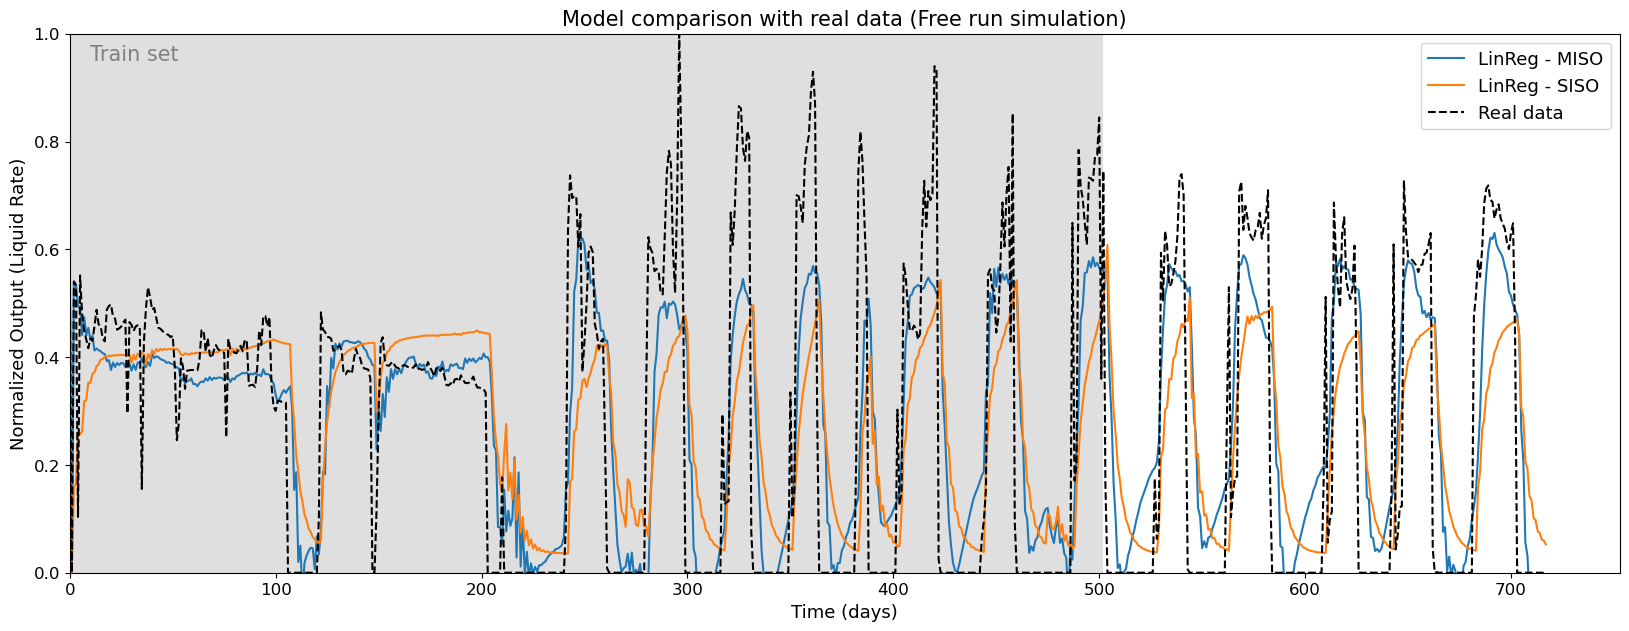
\includegraphics[width=6in]{images/LinReg_comparison_big.png}\label{linreg_comp}}
\hfil
%\subfloat[LinReg residuals auto-correlation comparison]{\includegraphics[width=3in]%{images/LinReg_correlation.png}\label{linreg_corr}}
%\hfil
\subfloat[PolyReg results comparison]{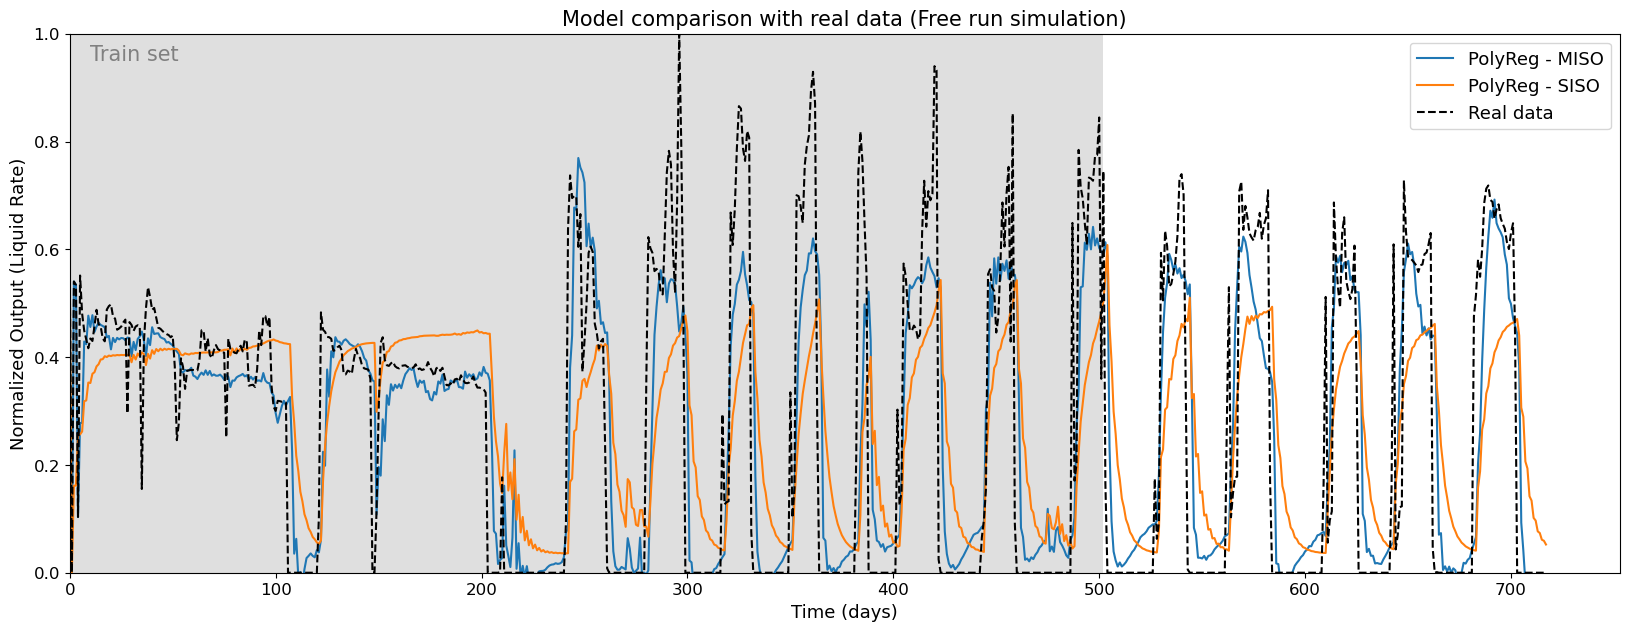
\includegraphics[width=6in]{images/PolyReg_comparison_big.png}\label{polyreg_comp}}
\hfil
%\subfloat[PolyReg residuals auto-correlation]{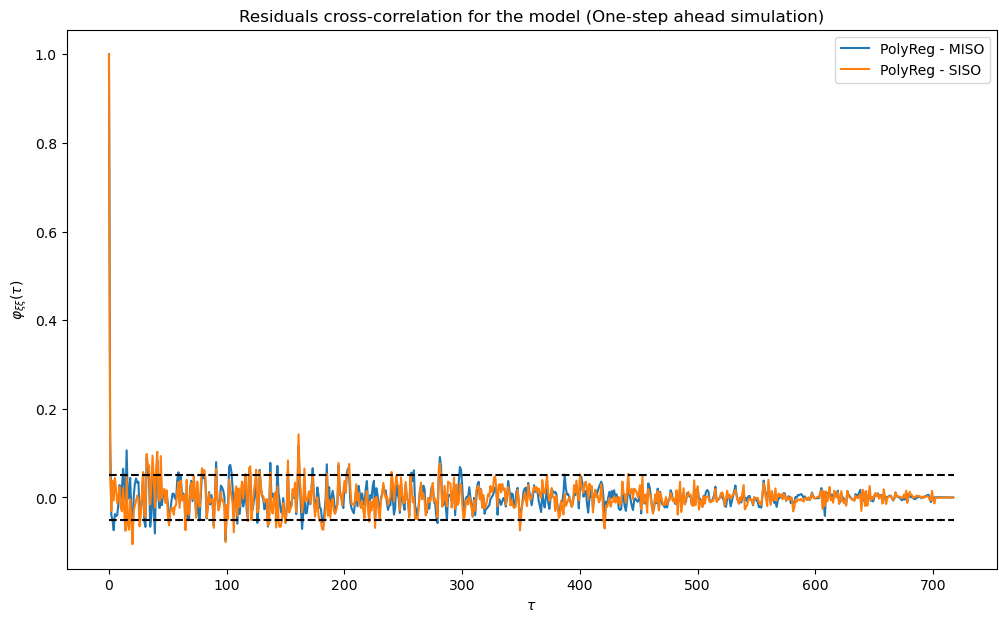
\includegraphics[width=3in]{images/PolyReg_correlation.png}\label{polyreg_corr}}
%\hfil
\subfloat[MLP results comparison]{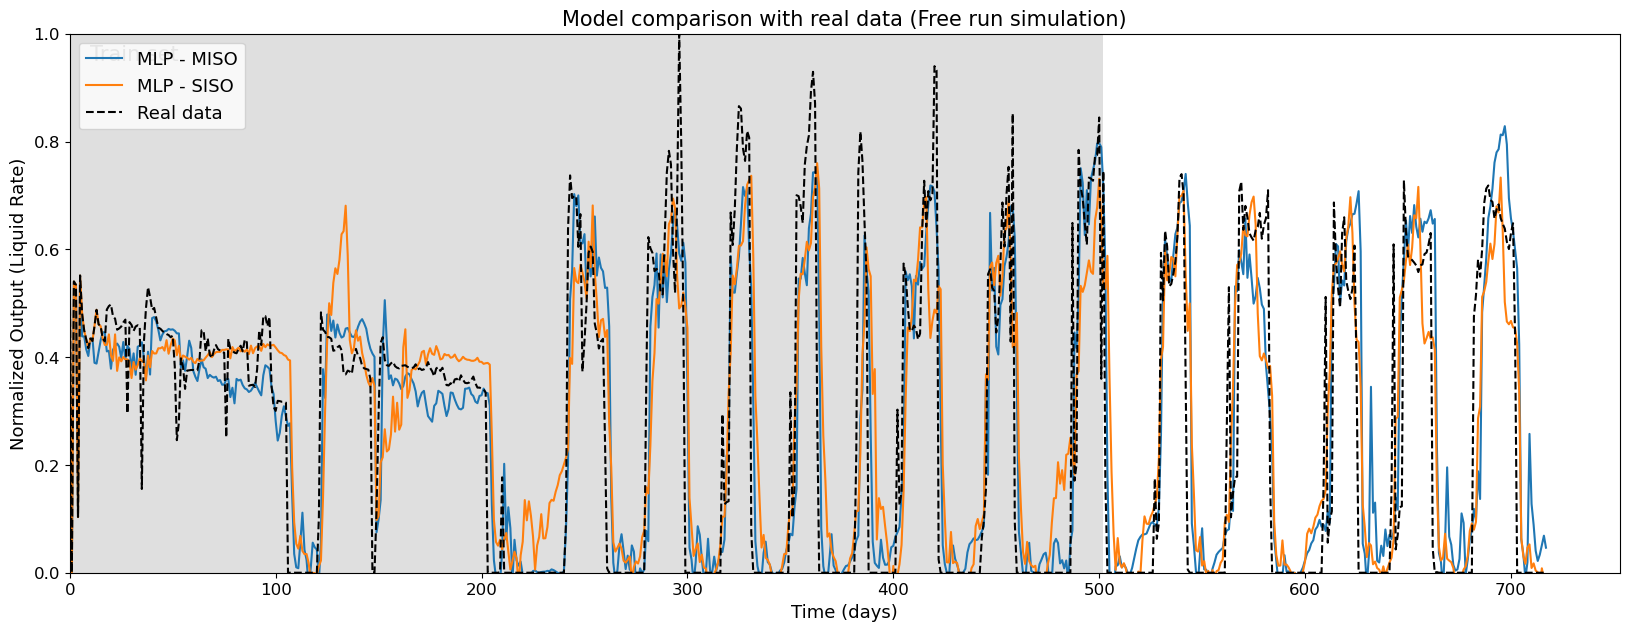
\includegraphics[width=6in]{images/MLP_comparison_big.png}\label{mlp_comp}}
\hfil
%\subfloat[MLP residuals auto-correlation]{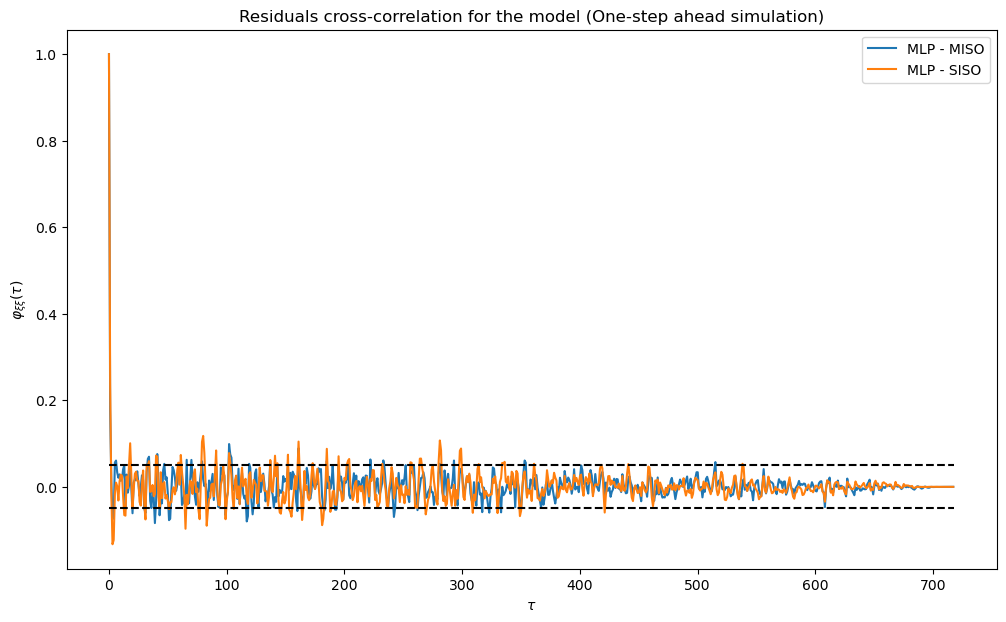
\includegraphics[width=3in]{images/MLP_correlation.png}\label{mlp_corr}}
%\hfil
\caption{Results achieved with the evaluated models}
\label{final_results}
\end{figure*}

\begin{table*}[htbp]
\caption{Metrics results for realized tests}
\begin{center}
\begin{tabular}{|c|c|c|c|c|c|c|c|c|c|c|}
\hline
\textbf{Method,}&\textbf{Best}&\multicolumn{4}{|c|}{\textbf{Train data}}&\multicolumn{4}{|c|}{\textbf{Total data}}&\textbf{Rank} \\
\cline{3-10} 
\textbf{Inputs} & \textbf{lag} & \textbf{\textit{R$^{\mathrm{2}}$ OSA}}& \textbf{\textit{R$^{\mathrm{2}}$ FS}}& \textbf{\textit{RMSE OSA}}& \textbf{\textit{RMSE FS}}& \textbf{\textit{R$^{\mathrm{2}}$ OSA}}& \textbf{\textit{R$^{\mathrm{2}}$ FS}} & \textbf{\textit{RMSE OSA}}& \textbf{\textit{RMSE FS}}& \\
\hline
\hline
ARX          &  4 & 0.803 & 0.795 & 0.117 & 0.170 & 0.585 & 0.592 & 0.124 & 0.175&4\\
%MISO    &&&&&&&&& \\
\hline
NARX         &  5 & 0.821 & 0.810 & 0.112 & 0.155 & 0.655 & 0.662 & 0.119 & 0.159&2\\
%MISO    &&&&&&&&& \\
\hline
MLP          &  6 & 0.898 & 0.852 & 0.084 & 0.139 & 0.723 & 0.688 & 0.105 & 0.153&1\\
\hline
Transformer  &  6 & 0.898 & 0.852 & 0.084 & 0.139 & 0.723 & 0.688 & 0.105 & 0.153&1\\
%MISO    &&&&&&&&& \\
\hline
\end{tabular}
\label{main_results}
\end{center}
\end{table*}

Another general comment that can be made by these results is that, as a general rule, the MISO approach, with the addition of information of the pressure and temperature sensors considerably improves the results of the error metrics, specially for the free-run simulations. In fact, by comparing the RMSE for the free-run simulations we can see reductions of the error as great as 5\% of the peak flow rate when adopting the MISO approach. This conclusion somehow agrees with the results presented by Li et al. in \cite{Li2019}, where to some extent cases with more input variables showed better error metrics even though it was not the case with the most extensive input space. It is also interesting to notice that this improvement is more significant on the more classical models (LinReg and PolyReg) than on the MLP case, indicating that the SISO approach using the MLP regressor shows good results to the point that it almost matches or outperforms the LinReg and PolyReg model on the MISO approach, being the third best model. This is a great advantage of the MLP model since it can obtain good results using only the choke size, the control variable effectively used to control the well production, as an input variable, making the model built using this regressor more robust to the loss of pressure and temperature sensors.

Analyzing the results for the LinReg and PolyReg models it is also interesting to notice that these two models do not show any differences for the SISO case, indicating that the importance of polynomial terms when the input space is essentially the choke opening and its lags is almost null. A stronger evidence of this behaviour is shown in table \ref{main_results}, where we can see that for the SISO approach, the LinReg and PolyReg obtained the same error metrics and the same optimal lag order, indicating that they converged for the same model. It is also interesting to notice by comparing these two models with the MLP model for the SISO case that the optimal lag order that they converged to was considerably lower than the one of the MLP model, which is another evidence of the poor performance of these models on the SISO approach since they lacked the ability of incorporating more data from the time series in order to improve their results.

Still looking on the fit time shown in table \ref{main_results}, it is important to notice that the MLP model has a significantly greater computational cost than the other models analyzed, with mean fit times at least 10 times greater than the other models. This is an important trade-off to have in mind since, depending on the amount of history data to fit and the number and range of hyperparameters to tune, it can have a considerable impact on the time demanded to build the model. In that aspect, te PolyReg model with MISO inputs is an interesting option to have in mind if computational time is an issue once it has relatively similar performance to the MLP model on the metrics, but a considerably lower fit time.

Analyzing now the randomized search and cross validation results, table \ref{mlp_results} shows the best hyperparameters found for the MLP regressor on the SISO and MISO cases. For the other models, the only parameter varied was the 'positive' parameter of the LinearRegressor, that showed the best results when set to True. It is interesting to notice that the MISO approach allows a significant reduction on the number of hidden units for the best model. It is also interesting to notice that the addition of more input data causes a reduction of the best lag from 17 on the SISO model to 6 on the MISO model. This change allows the reduction of the number of parameters of the MLP model from aroud 15000 on the SISO case for around 3000 on the MISO case, which also reflects on the mean fit time for the MLP model, as displayed on table \ref{main_results}.

\begin{table}[htbp]
\caption{Best parameters for MLP Randomized Search}
\begin{center}
\begin{tabular}{|c|c|c|}
\hline
\textbf{Parameter}&\multicolumn{2}{|c|}{\textbf{Value}} \\
\cline{2-3} 
\textbf{} & \textbf{\textit{SISO}} & \textbf{\textit{MISO}} \\
\hline
alpha                &           1.2e-3 &           1.4e-3  \\
\hline
batch\_size          &               64 &              128  \\
\hline
early\_stopping      &             True &            False  \\
\hline
hidden\_layer\_sizes & [80, 80, 60, 20] & [20, 40, 20, 40]  \\
\hline
tol                  &           1.4e-3 &           5.6e-6  \\
\hline
\end{tabular}
\label{mlp_results}
\end{center}
\end{table}


%\begin{table}[htbp]
%\caption{Mean fit time for the models evaluated}
%\begin{center}
%\begin{tabular}{|c|c|c|}
%\hline
%\textbf{Parameter}&\multicolumn{2}{|c|}{\textbf{Time (seconds)}} \\
%\cline{2-3} 
%\textbf{} & \textbf{\textit{SISO}} & \textbf{\textit{MISO}} \\
%\hline
%LinReg                &          1.09e-3 &            1.32e-3\\
%\hline
%PolyReg               &          1.53e-3 &            3.64e-2\\
%\hline
%MLP                   &          4.80e-1 &            3.67e-1\\
%\hline
%\end{tabular}
%\label{time_results}
%\end{center}
%\end{table}

Another important factor to consider while selecting a model is the model sensitivity to the input data. This can be evaluated by comparing the R$^2$ score of another metric of choice of the models when fitted with different input spaces during cross-validation. These results are shown on the figure \ref{cv_stats}, where a boxplot of the R$^2$ results for the validation folds is shown. Once again, it is clear that the MLP is a more adequate method since the dispersion of the metric is lower for all the cross-validation fits performed. This indicates that the MLP model is less sensitive to the selection of an specific train set. It is also interesting to notice that the use of MISO inputs reduces the dispersion of the data, indicating that the addition of more sensor data also helps the model to be less sensitive to the train set.

\begin{figure}[htbp]
\centerline{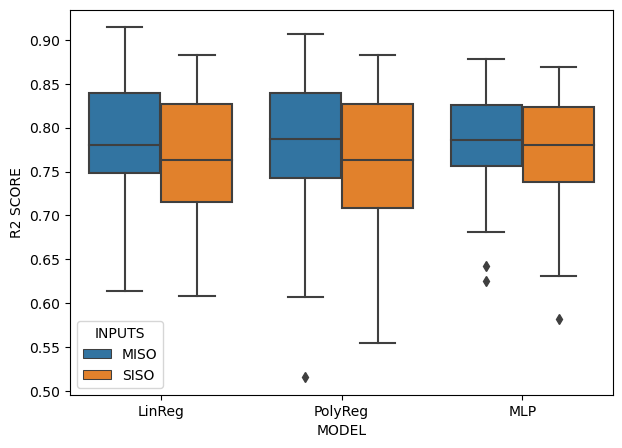
\includegraphics[width=3.5in]{images/boxplot_cv.png}}
\caption{Boxplot comparison of the R$^2$ metric for the three models evaluated during cross-validation}
\label{cv_stats}
\end{figure}

\section{Conclusion}\label{section_conclusion}

%\color{red}
%retomar brevemente as discussoes feitas na secao 4
%apontar trabalhos futuros
%\color{black}

This work applied a system identification approach to create a black box model of a production oil well. In search for the best model, this work built a python class capable of using any sklearn-compatible regressor in order to perform the system identification and chose the best model by following a grid search approach for lag order selection and a randomized search approach for hyperparameter selection on the regressor. This approach was tested with both single input (SISO) and multiple input (MISO).

From the three models tested in this work, it was possible to conclude that the Neural Network (MLP) model outperformed the ARX (LinReg) and NARX (PolyReg) models implemented in all metrics evaluated. Its performance was also superior regarding the dispersion of the R$^2$ score during cross-validation for both SISO and MISO approaches. The model also achieved similar performances to the other models on the MISO approach by using just the SISO approach, which indicates great prediction capability using only the active control variable available on the system.

The only downside found of the MLP model was its superior computational cost when compared with the other models, but for this case the PolyReg model with MISO approach could be a viable alternative, even though its performance is not as good as the MLP model according to the metrics adopted.

For future works, it is proposed to apply the same methodology to other sklearn regressors or more robust neural network architectures and frameworks, such as tensorflow or pytorch-implemented deep learning models, try the same methodology on other wells form the Volve dataset, on other datasets available or on the same well with additional information from other wells on the same reservoir, in order tho get possible interference effects between nearby wells. The application of Wiener-based estimators or spectral decomposition for this data is also part of possible future works.


% trigger a \newpage just before the given reference
% number - used to balance the columns on the last page
% adjust value as needed - may need to be readjusted if
% the document is modified later
%\IEEEtriggeratref{8}
% The "triggered" command can be changed if desired:
%\IEEEtriggercmd{\enlargethispage{-5in}}

% references section

% can use a bibliography generated by BibTeX as a .bbl file
% BibTeX documentation can be easily obtained at:
% http://mirror.ctan.org/biblio/bibtex/contrib/doc/
% The IEEEtran BibTeX style support page is at:
% http://www.michaelshell.org/tex/ieeetran/bibtex/
\bibliographystyle{IEEEtran}
% argument is your BibTeX string definitions and bibliography database(s)
% \bibliography{IEEEabrv,../bib/paper}
\bibliography{IEEEabrv,references}
%
% <OR> manually copy in the resultant .bbl file
% set second argument of \begin to the number of references
% (used to reserve space for the reference number labels box)
% \begin{thebibliography}{1}
% \bibitem{IEEEhowto:kopka}
% H.~Kopka and P.~W. Daly, \emph{A Guide to \LaTeX}, 3rd~ed.\hskip 1em plus
%   0.5em minus 0.4em\relax Harlow, England: Addison-Wesley, 1999.
% \end{thebibliography}




% that's all folks
\end{document}
